\documentclass[
	a4paper,
	oneside,
	BCOR = 10mm,
	DIV = 12,
	12pt,
	headings = normal,
]{scrartcl}

%%% Length calculations
\usepackage{calc}
%%%

%%% Support for color
\usepackage{xcolor}
\definecolor{lightblue}{HTML}{03A9F4}
\definecolor{red}{HTML}{F44336}
%%%

%%% Including graphics
\usepackage{graphicx}
%%%

%%% Font selection
\usepackage{fontspec}

\setromanfont{STIX Two Text}[
	SmallCapsFeatures = {LetterSpace = 8},
]

\setsansfont{IBM Plex Sans}[
	Scale = MatchUppercase,
]

\setmonofont{IBM Plex Mono}[
	Scale = MatchUppercase,
]
%%%

%%% Math typesetting
\usepackage{amsmath}

\usepackage{unicode-math}
\setmathfont{STIX Two Math}

\usepackage{IEEEtrantools}
%%%

%%% List settings
\usepackage{enumitem}
\setlist[enumerate]{
	label*      = {\arabic*.},
	left        = \parindent,
	topsep      = 0\baselineskip,
	parsep      = 0\baselineskip,
	noitemsep, % override itemsep
}
% List settings for levels 2–4
\setlist[enumerate, 2, 3, 4]{
	label*      = {\arabic*.},
	left        = 0em,
	topsep      = 0\baselineskip,
	parsep      = 0\baselineskip,
	noitemsep, % override itemsep
}

\setlist[itemize]{
	label*      = {—},
	left        = \parindent,
	topsep      = 0\baselineskip,
	parsep      = 0\baselineskip,
	itemsep     = 1\baselineskip,
	noitemsep, % override itemsep
}

\setlist[description]{
	font        = {\rmfamily\upshape\bfseries},
	topsep      = 1\baselineskip,
	parsep      = 0\baselineskip,
	itemsep     = 0\baselineskip,
}

%%%

%%% Structural elements typesetting
\setkomafont{pagenumber}{\rmfamily\upshape}
\setkomafont{disposition}{\rmfamily\bfseries}

% Sectioning
\RedeclareSectionCommand[
	beforeskip = -1\baselineskip,
	afterskip  = 1\baselineskip,
	font       = {\normalsize\bfseries\scshape},
]{section}

\RedeclareSectionCommand[
	beforeskip = -1\baselineskip,
	afterskip  = 1\baselineskip,
	font       = {\normalsize\bfseries\itshape},
]{subsection}

\RedeclareSectionCommand[
	beforeskip = -1\baselineskip,
	afterskip  = 1\baselineskip,
	font       = {\normalsize\bfseries},
]{subsubsection}

\RedeclareSectionCommand[
	beforeskip = -1\baselineskip,
	afterskip  = -0.5em,
	font       = {\normalsize\mdseries\scshape\addfontfeatures{Letters = {UppercaseSmallCaps}}},
]{paragraph}
%%%

%%% Typographic enhancements
\usepackage{microtype}
%%%

%%% Language-specific settings
\usepackage{polyglossia}
\setmainlanguage{ukrainian}
\setotherlanguages{english}
%%%

%%% Captions
\usepackage{caption}
\usepackage{subcaption}

%\DeclareCaptionLabelFormat{closing}{#2)}
%\captionsetup[subtable]{labelformat = closing}

%\captionsetup[subfigure]{labelformat = closing}

\captionsetup[table]{
	aboveskip = 0\baselineskip,
	belowskip = 0\baselineskip,
}

\captionsetup[figure]{
	aboveskip = 1\baselineskip,
	belowskip = 0\baselineskip,
}

\captionsetup[subfigure]{
	labelformat = simple,
	labelformat = brace,
	justification = RaggedRight,
	singlelinecheck = false,
}
%%%

%%% Hyphenated ragged typesetting
\usepackage{ragged2e}
%%%

%%% Table typesetting
\usepackage{booktabs}
\usepackage{longtable}

\usepackage{multirow}

\usepackage{array}
\newcolumntype{v}[1]{>{\RaggedRight\arraybackslash\hspace{0pt}}p{#1}}
\newcolumntype{b}[1]{>{\Centering\arraybackslash\hspace{0pt}}p{#1}}
\newcolumntype{n}[1]{>{\RaggedLeft\arraybackslash\hspace{0pt}}p{#1}}
%%%

%%% Drawing
\usepackage{tikz}
\usepackage{tikzscale}
\usetikzlibrary{positioning}
\usetikzlibrary{arrows.meta} % Stealth arrow tips
%%%

%%% SI units typesetting
\usepackage{siunitx}
\sisetup{
	output-decimal-marker = {,},
	exponent-product      = {\cdot},
	inter-unit-product    = \ensuremath{{} \cdot {}},
	per-mode              = symbol,
}
%%%

% Code Highlighting
\usepackage{minted}
\setmintedinline{
	style = bw,
	breaklines,
}

\newminted[bashterm]{text}{%
	autogobble,%
	breaklines,%
	style=bw,%
}

\newminted[codegeneric]{text}{%
	autogobble,%
	style=bw,%
	breaklines,%
	fontsize=\small,%
}

\newmintinline{bash}{%
}

\newmintinline[minttext]{text}{%
	breaklines,%
	breakanywhere,%
}

%%% Framing code listings
\usepackage{tcolorbox}
\tcbuselibrary{breakable}
\tcbuselibrary{minted}
\tcbuselibrary{skins}

% Text file listing
\newtcblisting[
	auto counter,
	list inside,
	number within = section,
]{listingplaintext}[3][]{%
	minted language = text,
	minted style    = bw,
	minted options  = {
		autogobble,
		linenos,
		tabsize = 4,
		breaklines,
		breakanywhere,
		fontsize = \footnotesize,
	},
	empty,
	sharp corners,
	coltitle = black,
	borderline horizontal = {1pt}{0pt}{black},
	titlerule = {0.5pt},
	titlerule style = {
		black,
	},
	toptitle = 0.3em,
	bottomtitle = 0.3em,
	before skip      = \intextsep,
	after  skip      = \intextsep,
	title            = {Лістинг \thetcbcounter: #2},
	list entry       = {\protect\numberline{\thetcbcounter}#2},
	left = 0em,
	right = 0em,
	%
	listing only,
	breakable,
	%
	label = {#3},%
}

\newtcblisting[
	use counter from = listingplaintext,
	list inside,
	number within = section,
]{listingpython}[3][]{%
	minted language = python,
	minted style    = bw,
	minted options  = {
		autogobble,
		linenos,
		tabsize = 4,
		breaklines,
		breakanywhere,
		fontsize = \footnotesize,
	},
	empty,
	sharp corners,
	coltitle = black,
	borderline horizontal = {1pt}{0pt}{black},
	titlerule = {0.5pt},
	titlerule style = {
		black,
	},
	toptitle = 0.3em,
	bottomtitle = 0.3em,
	before skip      = \intextsep,
	after  skip      = \intextsep,
	title            = {Лістинг \thetcbcounter: #2},
	list entry       = {\protect\numberline{\thetcbcounter}#2},
	left = 0em,
	right = 0em,
	%
	listing only,
	breakable,
	%
	label = {#3},
	%
	#1%
}

\newtcbinputlisting[
	use counter from = listingplaintext,
	list inside,
	number within = section
]{\inputpython}[4][]{%
	minted language = python,
	minted style    = bw,
	minted options  = {
		autogobble,
		linenos,
		tabsize = 4,
		breaklines,
		breakanywhere,
		fontsize = \footnotesize,
	},
	empty,
	sharp corners,
	coltitle = black,
	borderline horizontal = {1pt}{0pt}{black},
	titlerule = {0.5pt},
	titlerule style = {
		black,
	},
	toptitle = 0.3em,
	bottomtitle = 0.3em,
	before skip      = \intextsep,
	after  skip      = \intextsep,
	title            = {Лістинг \thetcbcounter: #3},
	list entry       = {\protect\numberline{\thetcbcounter}#3},
	left = 0em,
	right = 0em,
	%
	listing file={#2},
	listing only,
	breakable,
	%
	label = {#4}
}

% Linux command-line listing
\newtcblisting{linuxterm}%
{%
	% Syntax highlighing options
	listing only,%
	minted language = bash,%
	minted options={%
		autogobble,%
		linenos%
	},%
	% Presentation options
	empty,%
	%% Margins
	sharp corners,%
	toptitle = 0.0em,%
	bottomtitle = 0.0em,%
	left = 0em,%
	right = 0em,%
	before skip = \intextsep,%
	after skip = \intextsep,%
}

\newtcblisting{linuxtermout}%
{%
	% Syntax highlighing options
	listing only,%
	minted language = text,%
	minted options={%
		autogobble,%
		linenos%
	},%
	% Presentation options
	empty,%
	%% Margins
	sharp corners,%
	toptitle = 0.0em,%
	bottomtitle = 0.0em,%
	left = 0em,%
	right = 0em,%
	before skip = \intextsep,%
	after skip = \intextsep,%
}

% Dockerfile listings
\newtcblisting[
	use counter from = listingplaintext,
	list inside,
	number within = section,
]{listingdocker}[3][]{%
	minted language = dockerfile,
	minted style    = bw,
	minted options  = {
		autogobble,%
		linenos,
		tabsize = 4,
		breaklines,
		breakanywhere,
		fontsize = \footnotesize,
	},
	empty,
	sharp corners,
	coltitle = black,
	borderline horizontal = {1pt}{0pt}{black},
	titlerule = {0.5pt},
	titlerule style = {
		black,
	},
	toptitle = 0.3em,
	bottomtitle = 0.3em,
	before skip      = \intextsep,
	after  skip      = \intextsep,
	title            = {Лістинг \thetcbcounter: #2},
	list entry       = {\protect\numberline{\thetcbcounter}#2},
	left = 0em,
	right = 0em,
	%
	listing only,
	breakable,
	%
	label = {#3},%
}

% Docker Compose listings
\newtcblisting[
	use counter from = listingplaintext,
	list inside,
	number within = section,
]{listingdockercompose}[3][]{%
	minted language = yaml,
	minted style    = bw,
	minted options  = {
		autogobble,%
		linenos,
		tabsize = 4,
		breaklines,
		breakanywhere,
		fontsize = \footnotesize,
	},
	empty,
	sharp corners,
	coltitle = black,
	borderline horizontal = {1pt}{0pt}{black},
	titlerule = {0.5pt},
	titlerule style = {
		black,
	},
	toptitle = 0.3em,
	bottomtitle = 0.3em,
	before skip      = \intextsep,
	after  skip      = \intextsep,
	title            = {Лістинг \thetcbcounter: #2},
	list entry       = {\protect\numberline{\thetcbcounter}#2},
	left = 0em,
	right = 0em,
	%
	listing only,
	breakable,
	%
	label = {#3},%
}


% Customize minted line numbers
\renewcommand{\theFancyVerbLine}{\ttfamily\scriptsize\arabic{FancyVerbLine}}

%%%

%%% Typeset menus and keys
\usepackage{menukeys}[
	os=win,
]
%%%

%%% Links and hyperreferences
\usepackage{hyperref}
\hypersetup{
	bookmarksnumbered = true,
	colorlinks      = false,
	linkbordercolor = red,
	urlbordercolor  = lightblue,
	pdfborderstyle  = {/S/U/W 1.5},
}
%%%

%%% Length adjustment

% Set baselineskip, default is 14.5 pt
\linespread{1.068966} % ~15.5 pt
\setlength{\emergencystretch}{1em}
\setlength{\parindent}{1.5em}
\newlength{\gridunitwidth}
\setlength{\gridunitwidth}{\textwidth / 12}
%%%

%%% Custom commands
\newcommand{\allcaps}[1]{%
	{%
		\addfontfeatures{%
			Letters = UppercaseSmallCaps,
			LetterSpace = 8,%
		}%
		#1%
	}%
}
\newcommand{\filename}[1]{\texttt{#1}}
\newcommand{\progname}[1]{\texttt{#1}}
\newcommand{\commandname}[1]{\texttt{#1}}
\newcommand{\modulename}[1]{\texttt{#1}}
\newcommand{\transeng}[1]{{англ.}~\textit{\textenglish{#1}}}
%%%

%%% Custom math commands
\newcommand{\longvar}[1]{\mathit{#1}}
%%%

\begin{document}

\begin{titlepage}
		\begin{center}
			Міністерство освіти і~науки України\\
			Національний авіаційний університет\\
			Факультет кібербезпеки, комп'ютерної та програмної інженерії\\
			Кафедра комп'ютеризованих систем управління

			\vspace{\fill}
				Лабораторна робота №~1.3\\
				з~дисципліни «Захист інформації в комп'ютерних системах»\\
				на~тему «Резервне копіювання інформації»

			\vspace{\fill}

			\begin{flushright}
				Виконав:\\
				студент \allcaps{ФККПІ}\\
				групи \allcaps{СП}-425\\
				Рабін І.\,Р.\\
				Перевірила:\\
				Супрун О.\,М.
			\end{flushright}

			Київ 2019
		\end{center}
	\end{titlepage}

	\section{Мета роботи}
		Ознайомитись з основними принципами застосування резервного копіювання інформації у складі заходів захисту інформації.

	\section{Завдання роботи}
		Встановити програмне забезпечення резервного копіювання інформації та навчитись з ним працювати.

	\section{Хід роботи}
		\subsection{\textenglish{Unix}-утиліти резервного копіювання}
			\subsubsection{Утиліта~\textenglish{\progname{cpio}}}
				Утиліта~\textenglish{\progname{cpio}}~— це файловий архіватор загального призначення, зазвичай встановлений на \textenglish{Unix}-подібних операційних системах. Її ім'я утворене з фрази «скопіювати всередину і назовні»~(\transeng{copy in and out}), яка пояснює принцип її роботи: програма отримує дані зі стандартного вводу, оброблює їх і копіює у стандартний вивід.

				Утиліта~\textenglish{\progname{cpio}} підтримує такі формати: двійковий, стару версію~\textenglish{\allcaps{ASCII}}, нову версію \textenglish{\allcaps{ASCII}}, \textenglish{crc}, двійковий формат~\textenglish{\allcaps{HPUX}}, стару версію \textenglish{\allcaps{HPUX ASCII}}, стару версію~\textenglish{tar} та \textenglish{\allcaps{POSIX.1} tar}.

				У цієї утиліти є 3 основні функції: копіювати файли в архів, витягувати файли з архіву та копіювати файли в інше дерево директорій. Під час створення архіву, \textenglish{\progname{cpio}}  приймає список файлів у стандартний ввід, створює архів і надсилає його у стандартний вивід або у пристрій. Зазвичай використовують команди~\commandname{ls} або \commandname{find}, щоб створити список файлів. Наприклад, щоб створити архів~\filename{directory.cpio}, який містить файли поточної директорії, використовують таку команду:
				\begin{bashterm}
					ls | cpio -ov > directory.cpio
				\end{bashterm}
				Параметр~\minttext{-o} позначає, що необхідно створити архів, а параметр~\minttext{-p}~— що треба виводити назви файлів, які зараз архівуються. Символ~\minttext{>} перенаправляє створений архів зі стандартного виводу у необхідний файл.

				Щоб скопіювати усе дерево з поточної директорії, необхідно сформувати повний список файлів, наприклад, за допомогою команди~\commandname{find}:
				\begin{bashterm}
					find . -print -depth | cpio -ov > tree.cpio
				\end{bashterm}

				Щоб вилучити архів, створений утилітою~\textenglish{\progname{cpio}}, треба виконати таку команду:
				\begin{bashterm}
					cpio -iv < directory.cpio
				\end{bashterm}
				Параметр~\minttext{-i} вказує, що необхідно розпакувати файли з архіву. Якщо ж архів може містити дерево директорій, і необхідно створювати директорії, які містяться в дереві, необхідно вказати параметр~\minttext{-d}:
				\begin{bashterm}
					cpio -idv < tree.cpio
				\end{bashterm}
				Ця команда відтворить заархівоване дерево директорій у поточній директорій.

				Щоб скопіювати файли з поточної директорії в іншу, \textenglish{\progname{cpio}} використовують так:
				\begin{bashterm}
					find . -depth -print0 | cpio --null -pvd new-dir
				\end{bashterm}
				У цьому прикладі за допомогою команди \commandname{find} ми формуємо список файлів дерева директорій поточної директорії і вказуємо за допомогою параметра~\minttext{-0}, що їх необхідно розділяти за допомогою символів \textenglish{\allcaps{ASCII NUL}}. Потім, сформований список перенаправляється в утиліту~\progname{cpio}, яка за допомогою параметра~\minttext{--null} зчитує список, розділений вищезазначеними символами і створює передане дерево директорій у новій директорії~«\textenglish{new-dir}».

				Оскільки утиліта~\progname{cpio} заточена під роботу зі списками файлів як окремих одиниць, вона добре підходить для створення резервних копій індивідуальних файлів та дерев директорій.

			\subsubsection{Утиліта~\textenglish{\progname{dd}}}
				Утиліта~\progname{dd} призначена для конвертації і копіювання файлів. Її основний синтаксис такий:
				\begin{bashterm}
					dd [operand...]
				\end{bashterm}
				Операнди для цієї утиліти зазвичай виглядають так: \minttext{key=val}. Розглянемо синтаксис на прикладі використання програми.

				Основна функціональність програми заснована на копіюванні змісту одного файлу в інший. Наприклад, щоб скопіювати файл, утиліту використовують так:
				\begin{bashterm}
					dd if=/home/user/file1.txt of=file2.txt
				\end{bashterm}
				Тут операнд~\minttext{if=/home/user/file1.txt} означає, що вхідний файл знаходиться у директорії~\minttext{/home/user/file1.txt} і його необхідно скопіювати у поточну директорію, у файл~\minttext{file2.txt}. При такому використанні утиліта не перетворює дані, а лише повністю копіює їх як є.

				Утиліту~\progname{dd} можна використовувати для резервного копіювання головного завантажувального запису~(\transeng{Master Boot Record}). Він знаходиться у першому секторі диску, на якому він записаний, тому для цього використовують таку команду для диску~\minttext{/dev/sda}.
				\begin{bashterm}
					dd if=/dev/sda of=sda-mbr.img bs=512 count=1
				\end{bashterm}
				Тут параметр~\minttext{bs=512} встановлює розмір блоків вводу і виводу у 512 байт, а~\minttext{count=1} показує, що необхідно скопіювати 1 блок.

				Зробивши цю резервну копію, з неї можна відновити головний завантажувальний запис такою командою:
				\begin{bashterm}
					dd if=sda-mbr.img of=/dev/sda bs=512 count=1
				\end{bashterm}
				Тут джерелом є резервна копія, а призначення~— диск, з якого вона була знята. Таким чином можна відновити головний завантажувальний запис носія.

				Оскільки утиліта~\progname{dd} працює на низькому рівні, вона добре підходить для створення повних копій носіїв, на кшталт образів дисків, магнітних накопичувачів тощо.

			\subsubsection{Утиліта~\textenglish{\progname{scp}}}
				Утиліта~\progname{scp}~(\textenglish{Secure Copy}) призначена для безпечного копіювання файлів між двома хостами за допомогою протоколу~\textenglish{\allcaps{SCP}~(Secure Copy Protocol)}. Цей протокол організовує безпеку передачі даних, спираючись на протокол~\textenglish{\allcaps{SSH}~(Secure SHell)}, який використовує криптографічні інструменти для створення захищеного каналу передачі даних між джерелом і призначенням. Завдяки передачі даних захищеним каналом, неавторизовані сторони не можуть переглянути, зміст та інформацію про дані, що передаються.

				Припустимо, що необхідно зробити резервну копію файлу~\filename{file.txt}. Щоб скопіювати файл за допомогою утиліти~\progname{scp}, треба виконати таку команду:
				\begin{bashterm}
					scp file.txt alice@backup-01:/home/alice/bak/file.txt
				\end{bashterm}
				Ця команда скопіює файл~\filename{file.txt} у віддалений хост~\minttext{backup-01} від імені користувача~\minttext{alice} як файл~\minttext{/home/alice/bak/file.txt}.

				За допомогою цієї утиліти також можна копіювати файли з віддаленого хоста на локальний. Наприклад, щоб відновити файл~\minttext{file.txt} з резервної копії, треба виконати команду:
				\begin{bashterm}
					scp alice@backup-01:/home/alice/bak/file.txt file.txt
				\end{bashterm}
				Після цього на локальному комп'ютері з'явиться файл~\minttext{file.txt}, відтворений з резервної копії, відтвореної з локації~\minttext{backup-01}.

				Крім цього, можна копіювати файли між віддаленими хостами. Наприклад, щоб скопіювати резервну копію з першої локації в другу (синхронізувати їх), треба виконати таку команду:
				\begin{bashterm}
					scp alice@backup-01:/home/alice/bak/file.txt alice@backup-02:/home/alice/bak/file.txt
				\end{bashterm}
				Ця команда скопіює файл~\minttext{/home/alice/bak/file.txt} з локації~\minttext{backup-01} і помістить його за тим самим шляхом, але на хост~\minttext{backup-02}.

				Утиліта~\progname{scp} дозволяє копіювати директорії, вказавши параметр~\minttext{-r}:
				\begin{bashterm}
					scp -r /home/alice alice@backup-01:/home/alice/bak/
				\end{bashterm}
				Ця команда скопіює вміст домашньої директорії користувача~\minttext{alice} у першу локацію резервного копіювання~— \minttext{backup-01}.

				Отже, утиліта~\progname{scp} дозволяє безпечно копіювати файли і дерева директорій захищеним каналом, тому вона найкраще підходить для переміщення створених резервних копій у віддалені локації, наприклад, сервери резервних копій.

		\subsection{Засоби резервного копіювання~\textenglish{Windows}}
			\subsubsection{Засіб «Архівація файлів»}
				Засіб «Архівація файлів» дозволяє налаштувати періодичне резервне копіювання файлів, які знаходяться на накопичувачах комп'ютера. Щоб налаштувати архівацію файлів, необхідно використати її графічний інтерфейс, який знаходиться в меню~\menu{{Пуск} > {Панель керування} > {Архівація і відновлення}}. Для початку необхідно натиснути на кнопку «Налаштувати резервне копіювання»~(рис.~\ref{fig:01-archivation-01}).

				\begin{figure}[!htbp]
					\centering
					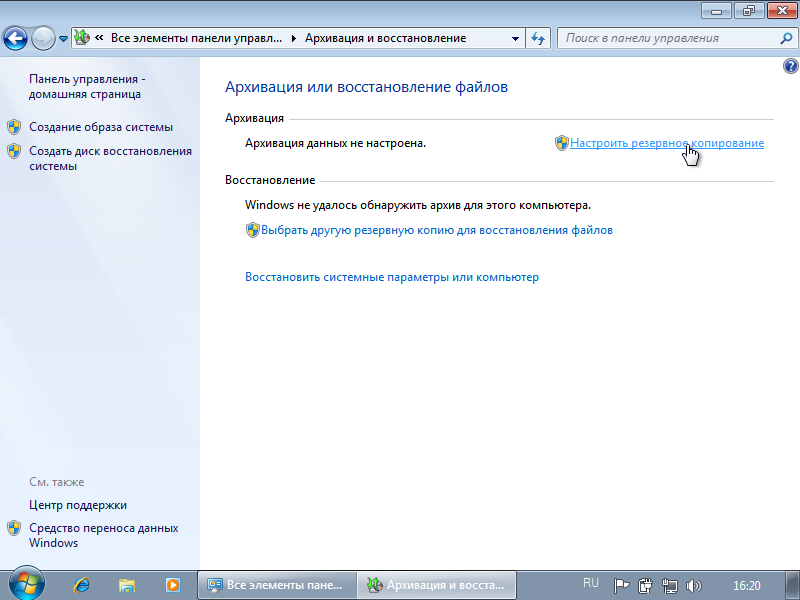
\includegraphics[height=11\baselineskip]{./assets/y04s01-infosec-lab-01-03-p01.png}
					\caption{Запуск налаштування резервного копіювання}
					\label{fig:01-archivation-01}
				\end{figure}

				Далі треба обрати місце призначення, куди будуть зберігатись резервні копії~(рис.~\ref{fig:01-archivation-02}). Можна обрати локальний накопичувач, наприклад, внутрішній або зовнішній жорсткий диск, оптичний диск, флеш-накопичувач чи віддалені накопичувачі, які знаходяться у мережі.

				\begin{figure}[!htbp]
					\centering
					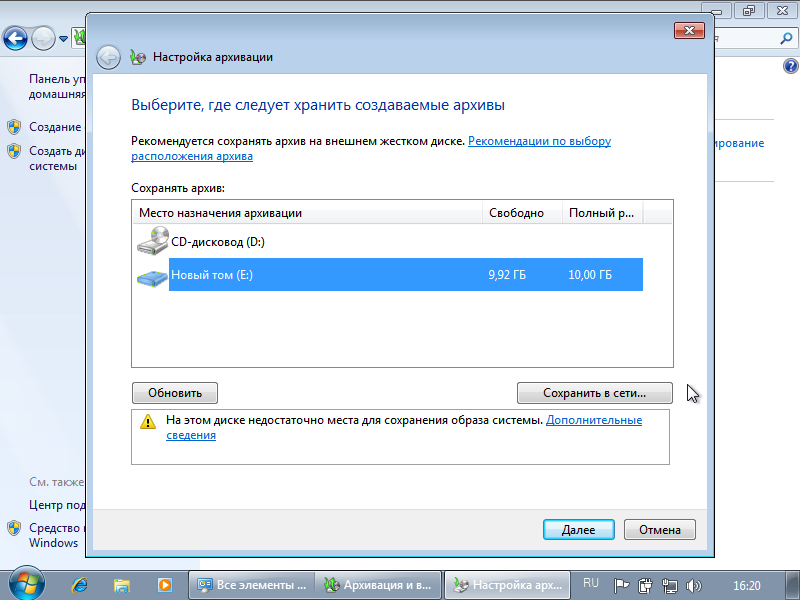
\includegraphics[height=12\baselineskip]{./assets/y04s01-infosec-lab-01-03-p02.png}
					\caption{Вибір місця збереження резервної копії}
					\label{fig:01-archivation-02}
				\end{figure}

				Після того, як користувач обрав місце для зберігання резервних копій, йому треба вибрати, яким чином обирати файли для резервного копіювання~(рис.~\ref{fig:01-archivation-03}). Засіб «Архівація файлів» дозволяє автоматично обирати файли для резервного копіювання на розсуд операційної системи або ж обирати їх вручну.

				\begin{figure}[!htbp]
					\centering
					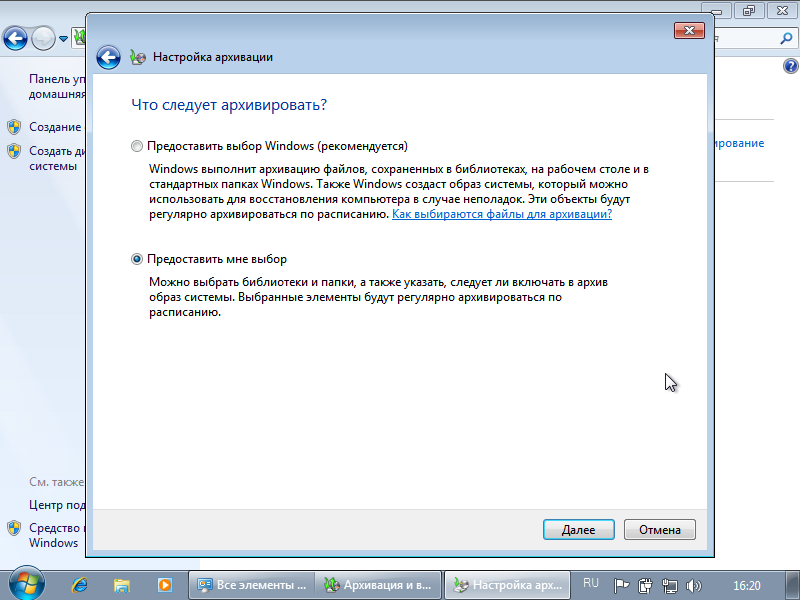
\includegraphics[height=12\baselineskip]{./assets/y04s01-infosec-lab-01-03-p03.png}
					\caption{Варіанти способу вибору файлів для резервної копії}
					\label{fig:01-archivation-03}
				\end{figure}

				Якщо користувач обрав ручний вибір файлів, він має обрати, які файли зберігати у резервних копіях~(рис.~\ref{fig:01-archivation-04}). Засіб дозволяє обрати стандартні розташування операційної системи та директорії, які знаходяться на доступних накопичувачах. Також можна до резервної копії можна додати образ операційної системи, який дозволить відновити її у разі пошкодження системних файлів, але і займає декілька гігабайтів пам'яті.

				\begin{figure}[!htbp]
					\centering
					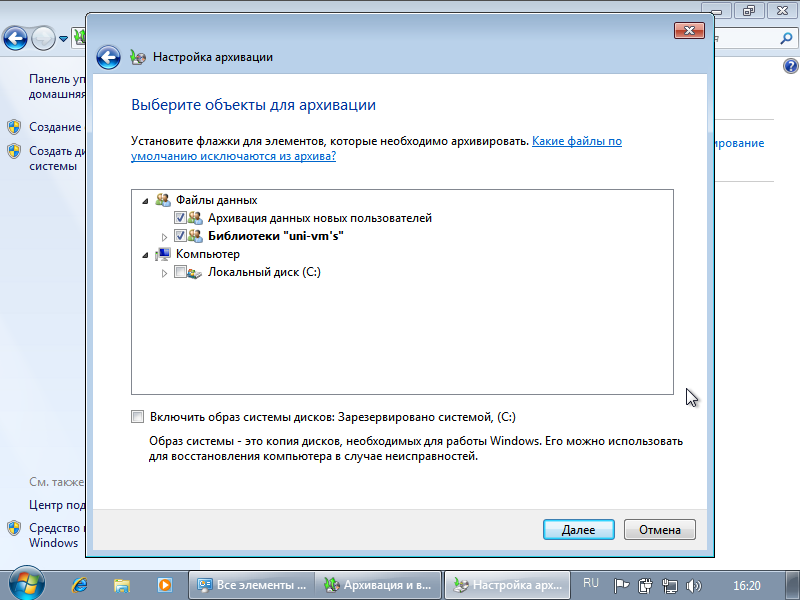
\includegraphics[height=12\baselineskip]{./assets/y04s01-infosec-lab-01-03-p04.png}
					\caption{Вибір файлів, які ввійдуть у резервну копію}
					\label{fig:01-archivation-04}
				\end{figure}

				Після вибору файлів засіб пропонує користувачу перевірити, які файли будуть включені у резервну копію, які налаштування будуть використані, щоб її створити, та задати розклад її запуску~(рис.~\ref{fig:01-archivation-05}). Щоб змінити розклад, необхідно натиснути на пункт~«Змінити розклад» і обрати бажану періодичність.

				\begin{figure}[!htbp]
					\centering
					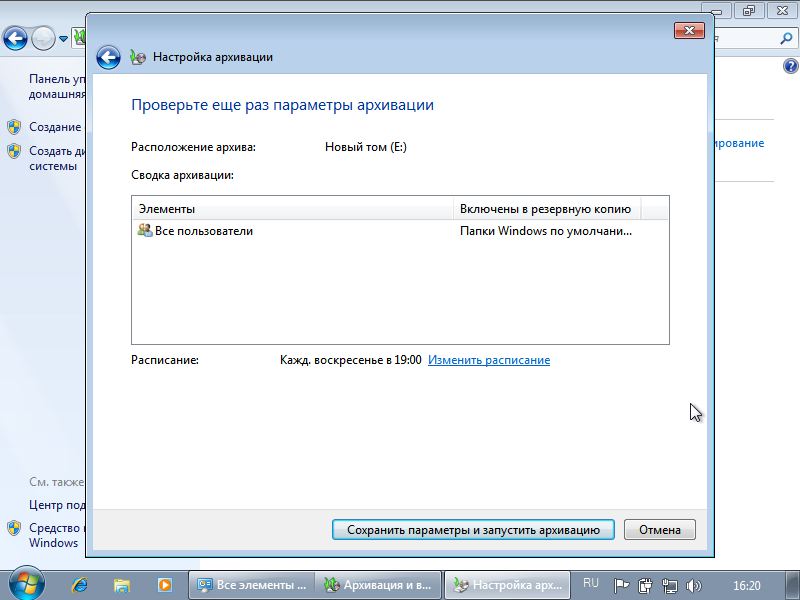
\includegraphics[height=12\baselineskip]{./assets/y04s01-infosec-lab-01-03-p05.png}
					\caption{Перегляд обраних налаштувань}
					\label{fig:01-archivation-05}
				\end{figure}

				Коли налаштування збережені, засіб запустить архівацію і відобразить відповідні змінні у своєму вікні~(рис.~\ref{fig:01-archivation-06}).

				\begin{figure}[!htbp]
					\centering
					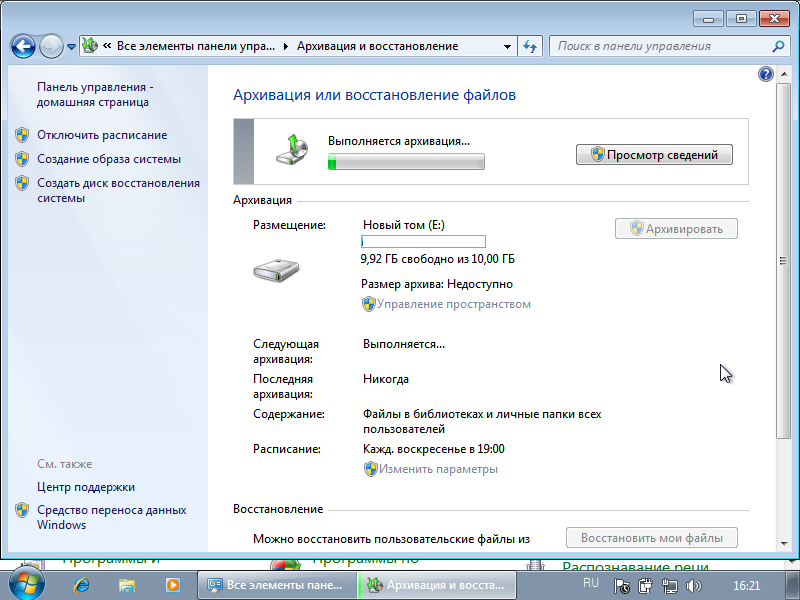
\includegraphics[height=12\baselineskip]{./assets/y04s01-infosec-lab-01-03-p06.png}
					\caption{Результат налаштування архівації}
					\label{fig:01-archivation-06}
				\end{figure}

				Отже, ми розглянули, як користувач може налаштувати періодичне створення резервних копій файлів, які зберігаються на накопичувачах його комп'ютера за допомогою засобу «Архівація файлів».

			\subsubsection{Засіб «Архівація образу системи»}
				Засіб «Архівація образу системи» дозволяє користувачу створити резервну копію образу операційної системи, щоб мати змогу відновити її, якщо її системні файли будуть пошкоджені. Щоб запустити цей засіб, необхідно перейти в меню~\menu{{Пуск} > {Панель керування} > {Архівація і відновлення}} і обрати пункт~«Створення образу системи»~(рис.~\ref{fig:02-system-img-01}).

				\begin{figure}[!htbp]
					\centering
					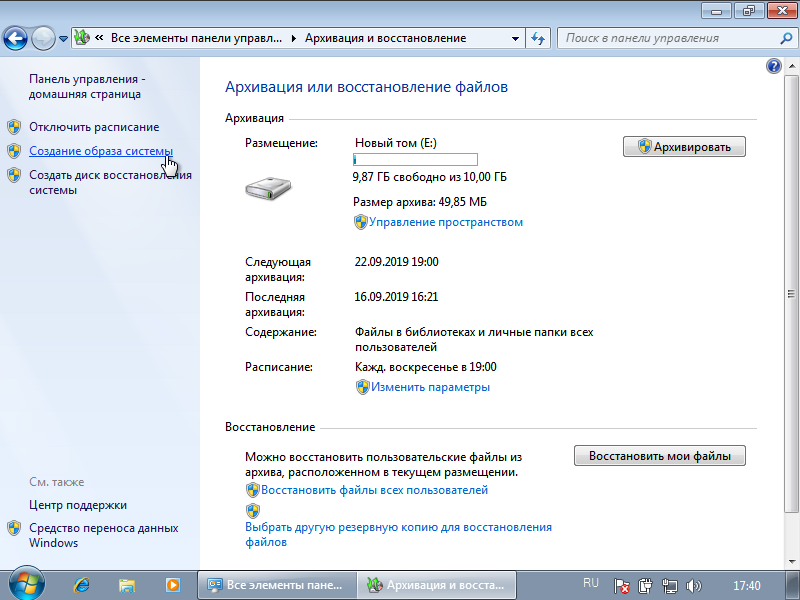
\includegraphics[height=11\baselineskip]{./assets/y04s01-infosec-lab-01-03-p07.png}
					\caption{Кнопка запуску архівації образу системи}
					\label{fig:02-system-img-01}
				\end{figure}

				Після того, як користувач натисне на кнопку, відкриється вікно створення образу системи~(рис.~\ref{fig:02-system-img-02}). На його першому екрані необхідно вказати, де треба зберігати образ системи. Користувач має обрати місце збереження і натиснути кнопку «Далі».

				\begin{figure}[!htbp]
					\centering
					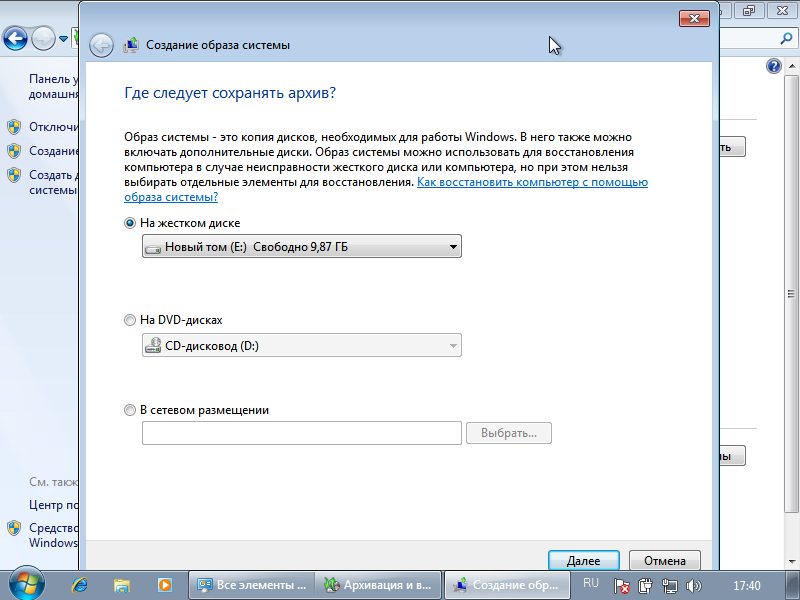
\includegraphics[height=12\baselineskip]{./assets/y04s01-infosec-lab-01-03-p08.png}
					\caption{Вибір місця, де зберігатиметься образ системи}
					\label{fig:02-system-img-02}
				\end{figure}

				Коли користувач обрав місце збереження резервної копії і натиснув кнопку «Далі», засіб перейде до наступного екрана~— підтвердження параметрів архівації~(рис.~\ref{fig:02-system-img-03}). Щоб підтвердити параметри архівації, необхідно натиснути кнопку «Архівувати».

				\begin{figure}[!htbp]
					\centering
					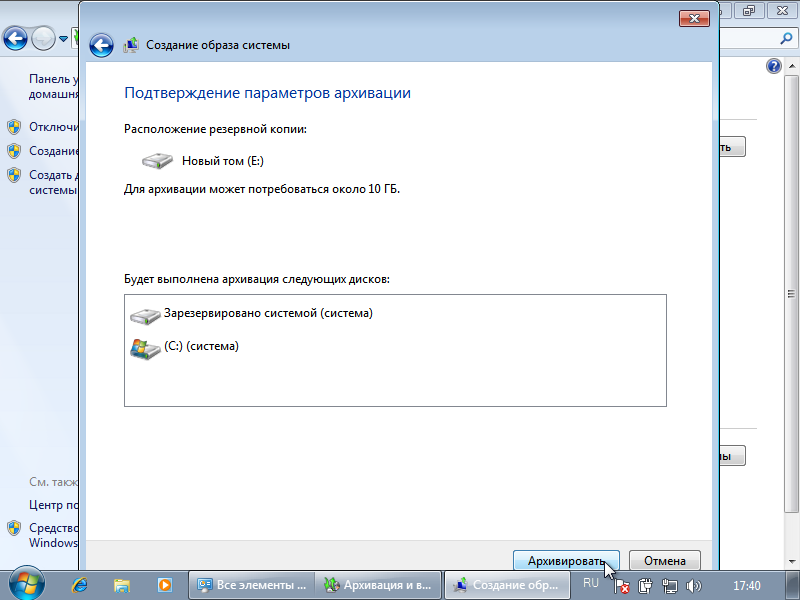
\includegraphics[height=12\baselineskip]{./assets/y04s01-infosec-lab-01-03-p09.png}
					\caption{Запуск архівації}
					\label{fig:02-system-img-03}
				\end{figure}

				Після того, як архівація завершиться, засіб запропонує створити диск відновлення системи~— записати резервну інформацію на носій, за допомогою якого можна буде відновити операційну систему, якщо вона пошкодиться і вийде з ладу~(рис.~\ref{fig:02-system-img-04}). В реальній ситуації доцільно створити цей диск, але в рамках даної лабораторної роботи це не потрібно.

				\begin{figure}[!htbp]
					\centering
					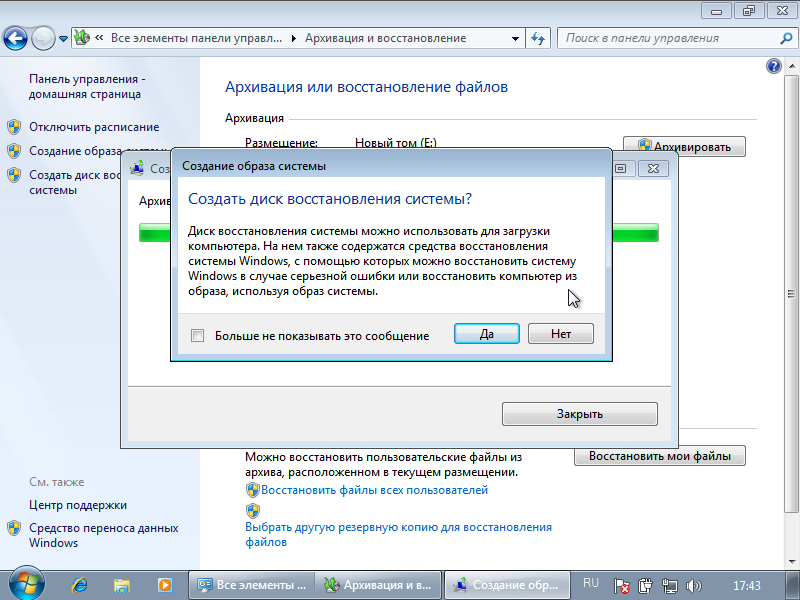
\includegraphics[height=12\baselineskip]{./assets/y04s01-infosec-lab-01-03-p11.png}
					\caption{Архівація завершена. Засіб пропонує створити диск відновлення системи}
					\label{fig:02-system-img-04}
				\end{figure}

				Тепер образ системи створений. Отже, ми розглянули, як створити резервний образ операційної системи, щоб відновити її у разі виникнення неполадок.

			\subsubsection{Засіб «Попередні версії»}
				Засіб «Попередні версії» призначений для відновлення попередніх версій файлів із точок відновлення~\textenglish{Windows} або резервних копій, створених за допомогою архівації~\textenglish{Windows}. Щоб скористатись можливостями засобу «Попередні версії», треба обрати файл, попередню версію якого треба відновити, викликати його контекстне меню і обрати пункт «Властивості». Після натискання кнопки «Властивості» відкриється вікно властивостей файлу. У вікні властивостей треба перейти на вкладку «Попередні версії», в якій будуть зображені всі доступні попередні версії файлу~(рис.~\ref{subfig:03-previous-versions-01-01}).

				Щоб відновити файл до його попередньої версії, обираємо необхідну версію та натискаємо кнопку «Відновити». Відкриється вікно відновлення файла, в якому з'явиться попередження, що файл з таким ім'ям вже існує~(рис.~\ref{subfig:03-previous-versions-01-02}). Щоб замінити файл, варто вибрати варіант «Копіювати із заміною», щоб зберегти обидві версії~— «Копіювати, але зберегти обидва файли». Після вибору стратегії копіювання файл буде відновлений~(рис.~\ref{subfig:03-previous-versions-01-03}).

				\begin{figure}[!htbp]
					%\centering
					\begin{subfigure}[b]{5\gridunitwidth}
						%\centering
						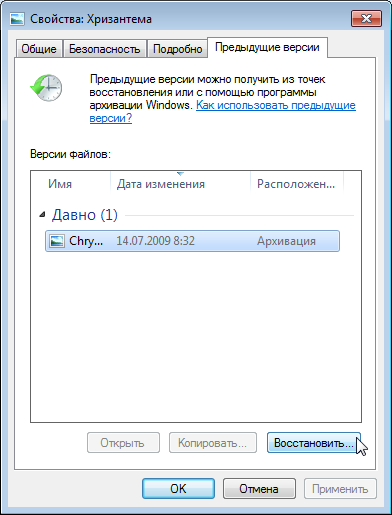
\includegraphics[height=12\baselineskip]{./assets/y04s01-infosec-lab-01-03-p13.png}
						% \caption{Вкладка «Попередні версії»}
						\caption{}
						\label{subfig:03-previous-versions-01-01}
					\end{subfigure}%
					\hspace{2\gridunitwidth}%
					\begin{subfigure}[b]{5\gridunitwidth}
						%\centering
						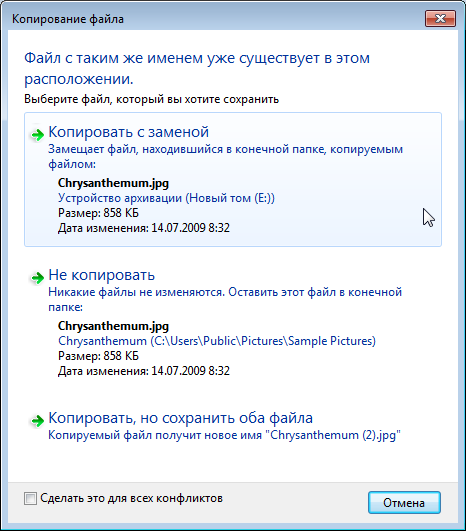
\includegraphics[height=12\baselineskip]{./assets/y04s01-infosec-lab-01-03-p14.png}
						\caption{}
						\label{subfig:03-previous-versions-01-02}
					\end{subfigure}

					\begin{subfigure}[b]{7\gridunitwidth}
						%\centering
						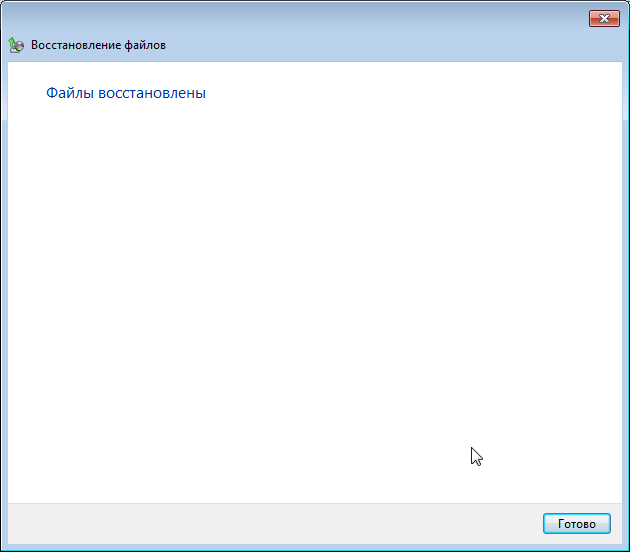
\includegraphics[width=\columnwidth]{./assets/y04s01-infosec-lab-01-03-p15.png}
						\caption{}
						\label{subfig:03-previous-versions-01-03}
					\end{subfigure}
					\caption{Відновлення файлу попередньої версії}
					\label{fig:03-previous-versions-01}
				\end{figure}

				Отже, ми розглянули, які можливості надає засіб «Попередні версії», а саме як створюються версії файлів і як відновити файл до його попередньої версії.

			\subsubsection{Засіб «Відновлення системи»}
				Засіб «Відновлення системи» дає користувачу можливість відновити певні компоненти системи за допомогою резервних копій, створених її засобами. Зазвичай ці точки відновлення створюються під час встановлення драйверів, важливих програм або користувач може створити їх вручну. Щоб відновити систему, необхідно відкрити засіб і слідувати його настановам~(рис.~\ref{fig:04-sysrestore-01}).

				\begin{figure}[!htbp]
					%\centering
					\begin{subfigure}[b]{5.5\gridunitwidth}
						%\centering
						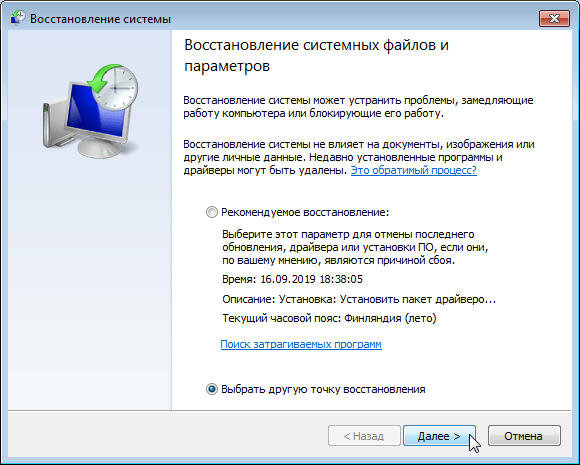
\includegraphics[width=\columnwidth]{./assets/y04s01-infosec-lab-01-03-p16.png}
						% \caption{Вкладка «Попередні версії»}
						\caption{}
						\label{subfig:04-sysrestore-01-01}
					\end{subfigure}%
					\hspace{1\gridunitwidth}%
					\begin{subfigure}[b]{5.5\gridunitwidth}
						%\centering
						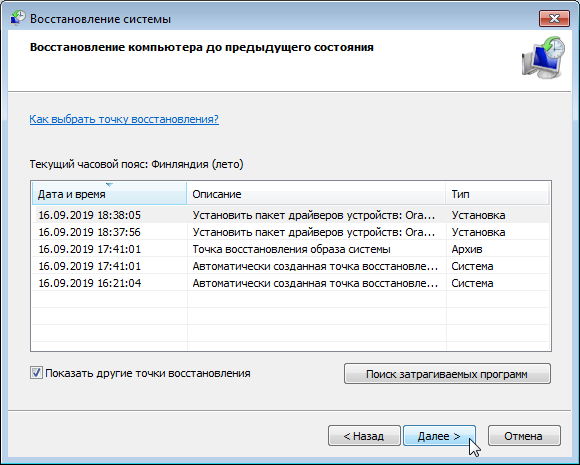
\includegraphics[width=\columnwidth]{./assets/y04s01-infosec-lab-01-03-p17.png}
						\caption{}
						\label{subfig:04-sysrestore-01-02}
					\end{subfigure}

					\begin{subfigure}[b]{5.5\gridunitwidth}
						%\centering
						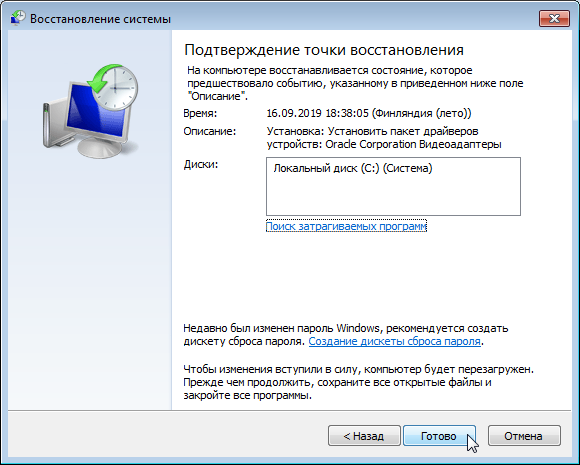
\includegraphics[width=\columnwidth]{./assets/y04s01-infosec-lab-01-03-p18.png}
						\caption{}
						\label{subfig:04-sysrestore-01-03}
					\end{subfigure}
					\caption{Відновлення системи}
					\label{fig:04-sysrestore-01}
				\end{figure}

				Після того, як користувач натисне кнопку «Готово», операційна система запустить відновлення за обраною резервною копією (точкою відновлення) і поверне файли у той вигляд, який вони мали на момент створення обраної копії.

				Отже, ми розглянули, як відновити операційну систему за допомогою засобу «Відновлення системи» і створених для нього точок відновлення.

		\subsection{Дослідження програми~«\textenglish{Acronis TrueImage}»}
			Програма~\textenglish{Acronis TrueImage}~— це програма призначена для створення резервних копій, яка запускається із завантажувального диску. Розглянемо процес її роботи.

			\subsubsection{Створення резервної копії за~допомогою завантажувального диска~\textenglish{Acronis True Image 2014}}
			\label{ssec:acronis-true-image-2014-backup}
				Налаштовуємо комп'ютер на завантаження з диску~\textenglish{Acronis True Image 2014} та перезавантажуємо його. У з'явившомуся меню обираємо пункт~\textenglish{«Acronis True Image 2014»} та натискаємо на нього. Виконалось завантаження необхідної підсистеми. Для створення резервної копії системи обираємо підпункт \menu{{Резервне копіювання} > {Диски}}, позначаємо системний диск \textenglish{C:}, та натискаємо на кнопку «Далі». У з'явившомуся вікні «Цільовий архів резервних копій» обираємо пункт «Створити новий архів резервних копій», обираємо шлях для збереження копії та натискаємо кнопку «Далі». Перевіряємо деталі резервного копіювання у з'явившомуся вікні та натискаємо кнопку «Приступити»~— розпочнеться процес резервного копіювання~(рис.~\ref{subfig:02-01-acronis-true-image-disk-backup-inprocess}). Після закінчення процесу програма звітує про успішне виконання~(рис.~\ref{subfig:02-01-acronis-true-image-disk-backup-res}).

				\begin{figure}[!htbp]
					\begin{subfigure}{5.5\gridunitwidth}
						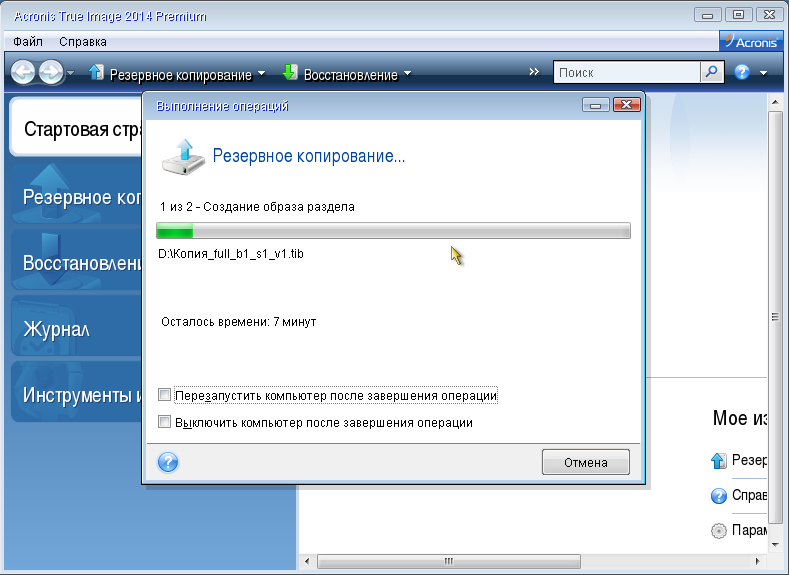
\includegraphics[width = \columnwidth]{./assets/y03s01-pcdiag-lab-04-p03.png}
						\caption{}
						\label{subfig:02-01-acronis-true-image-disk-backup-inprocess}
					\end{subfigure}%
					\hspace{1\gridunitwidth}%
					\begin{subfigure}{5.5\gridunitwidth}
						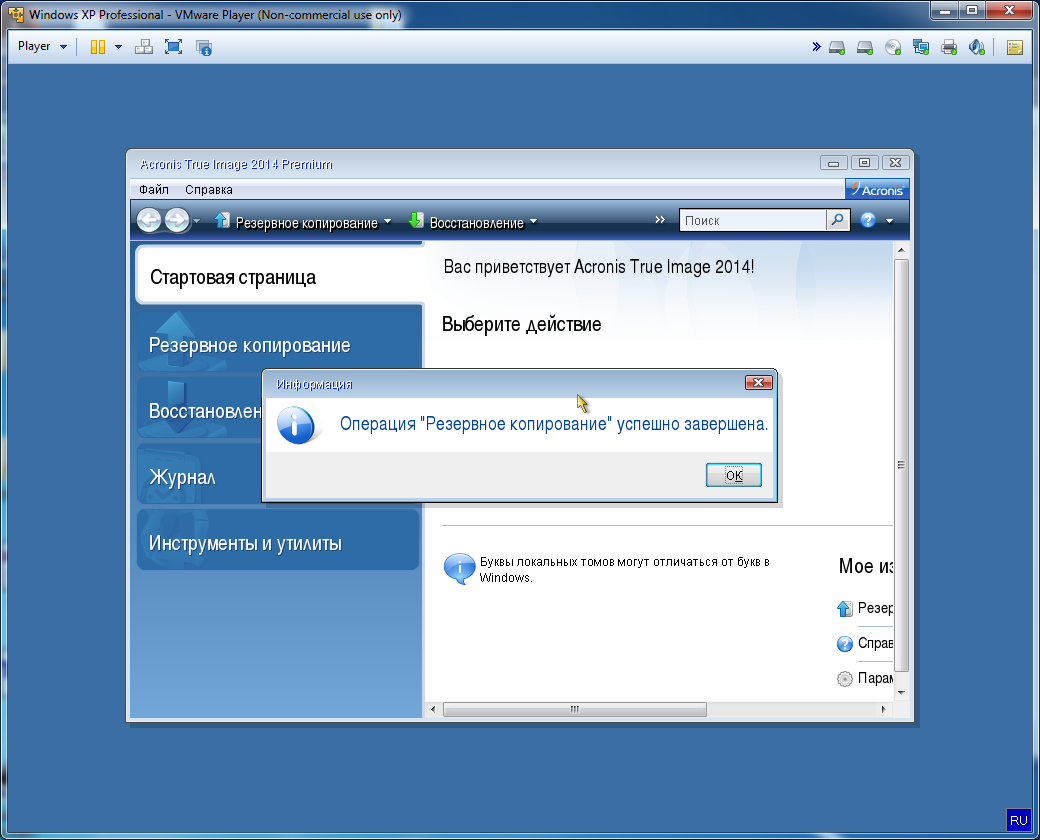
\includegraphics[width = \columnwidth]{./assets/y03s01-pcdiag-lab-04-p04.png}
						\caption{}
						\label{subfig:02-01-acronis-true-image-disk-backup-res}
					\end{subfigure}%
					\caption{Результат створення резервної копії завантажувальним диском~\textenglish{Acronis True Image 2014}}
					\label{fig:02-acronis-true-image-disk-backup-res}
				\end{figure}

				Отже, ми покроково розглянули, як створити резервну копію даних за допомогою програми~\textenglish{Acronis True Image}.

			\subsubsection{Відновлення резервної копії за~допомогою завантажувального диска~\textenglish{Acronis True Image 2014}}
				Повертаємось до стартової сторінки~\textenglish{Acronis True Image 2014} та обираємо підпункт \menu{{Відновлення} > {Диски}}. Обираємо резервну копію, створену у підпункті~\ref{ssec:acronis-true-image-2014-backup} та натискаємо «Далі». Встановлюємо режим «Відновити диски чи розділи», натискаємо «Далі». У вікні, що з'явилось, обираємо елементи для встановлення та натискаємо «Далі». Після перевірки обраних налаштувань запускаємо процес відновлення~(рис.~\ref{fig:03-acronis-true-image-disk-restore}).

				\begin{figure}[!htbp]
					\begin{subfigure}{5.5\gridunitwidth}
						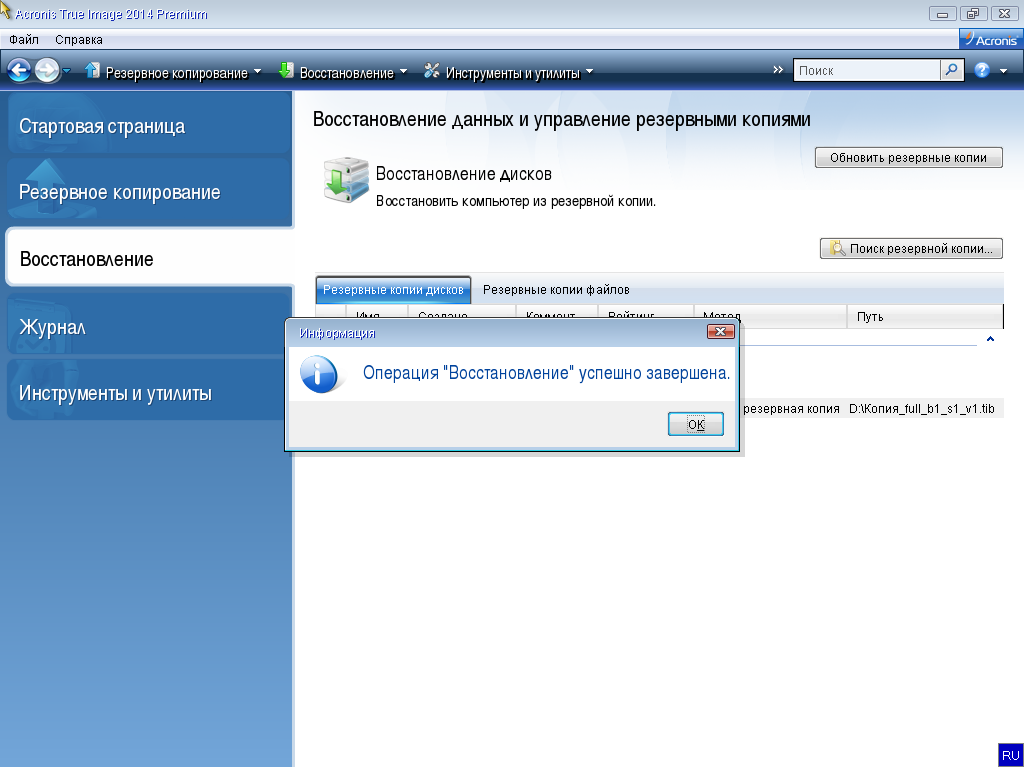
\includegraphics[width = \columnwidth]{./assets/y03s01-pcdiag-lab-04-p05.png}
						\caption{}
						\label{subfig:03-01-acronis-true-image-disk-restore-inprocess}
					\end{subfigure}%
					\hspace{1\gridunitwidth}%
					\begin{subfigure}{5.5\gridunitwidth}
						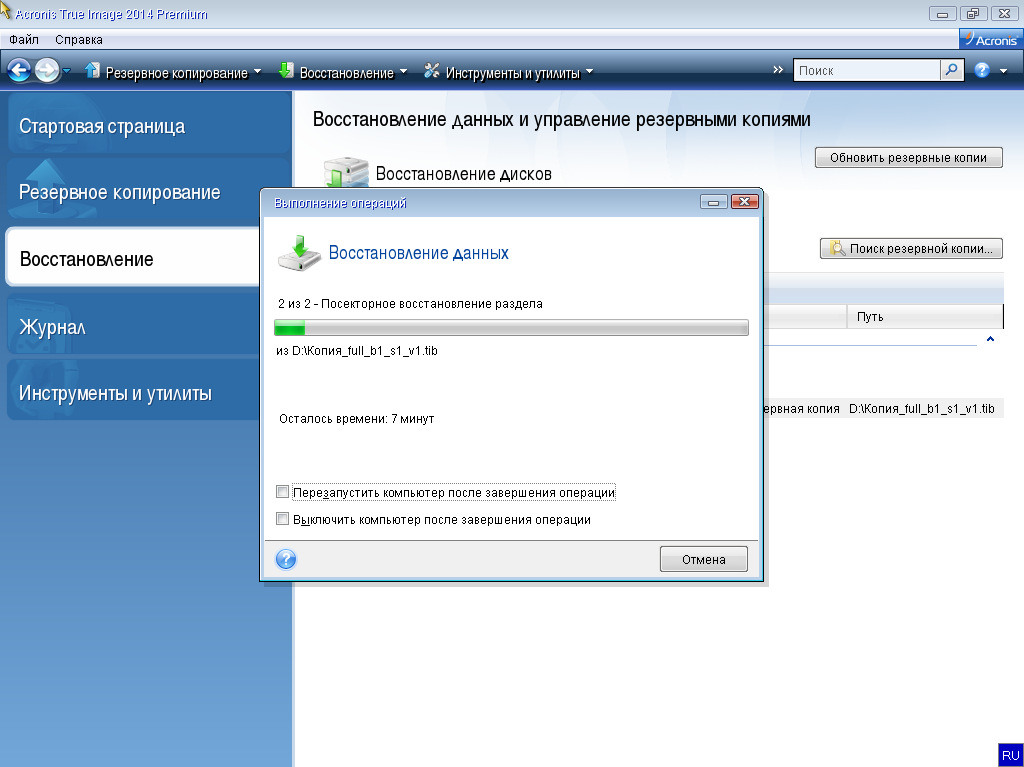
\includegraphics[width = \columnwidth]{./assets/y03s01-pcdiag-lab-04-p06.png}
						\caption{}
						\label{subfig:02-01-acronis-true-image-disk-restore-res}
					\end{subfigure}%
					\caption{Результат відновлення резервної копії завантажувальним диском~\textenglish{Acronis True Image 2014}}
					\label{fig:03-acronis-true-image-disk-restore}
				\end{figure}

				В результаті ми розглянули, як відновити дані зі створеної резервної копії за допомогою програми~\textenglish{Acronis True Image}.

		\subsection{Ознайомлення з програмою~«\textenglish{BackupPC}»}
			Програма~«\textenglish{BackupPC}» — це система резервного копіювання для операційних систем \textenglish{Unix, Linux, Windows} і \textenglish{macOS}. Вона написана мовою програмування~\textenglish{perl}, вилучає дані резервних копій протоколом~\textenglish{\allcaps{SMB}} за допомогою утиліт~\textenglish{Samba}, \textenglish{tar} через протоколи~\textenglish{\allcaps{SSH}, \allcaps{RSH}, \allcaps{NFS}} або~\textenglish{rsync}.

			Програма~\textenglish{BackupPC} має такі характеристики:
			\begin{enumerate}
				\item Використовує розумну систему пулінгу, яка зменшує використання дискового простору і часу його використання завдяки тому, що система зберігає лише одну копію ідентичних файлів, які містяться у декількох резервних копіях.
				\item Підтримує стиснення файлів.
				\item Не потребує установки програмного забезпечення на стороні клієнта, так як вона використовує стандартні і розповсюджені протоколи.
				\item Має потужний веб-інтерфейс, який дозволяє адміністраторам управляти системою, а користувачам~— переглядати і відновлювати файли з резервних копій~(рис.~\ref{fig:04-backuppc-01-01}, \ref{fig:04-backuppc-01-02}, \ref{fig:04-backuppc-01-03}, \ref{fig:04-backuppc-01-04}, \ref{fig:04-backuppc-01-05}).
				\item Підтримує як пряме відновлення, так і можливість скачати резервну копію у вигляді архіва.
				\item Підтримує мобільні середовища, в яких клієнти лише тимчасово підключені до мережі і мають динамічні адреси.
				\item Надає можливість гнучкого налаштування, зокрема створення декількох резервних копій паралельно, вибору змісту резервних копій, різноманітні розклади для повних і інкрементальних резервних копі тощо.
				\item Протестована на різних операційних системах, зокрема: \textenglish{Linux, Freenix, Solaris, Linux, Windows 95, 98, 200, \allcaps{XP}}.
				\item Має відкритий початковий код.
			\end{enumerate}
			Такий набір характеристик робить цю програму повноцінним рішенням для створення резервних копій не лише для звичайних користувачів комп'ютерів, а і для систем бізнес-класу з підвищеними вимогами.

			\begin{figure}[!htbp]
				\centering
				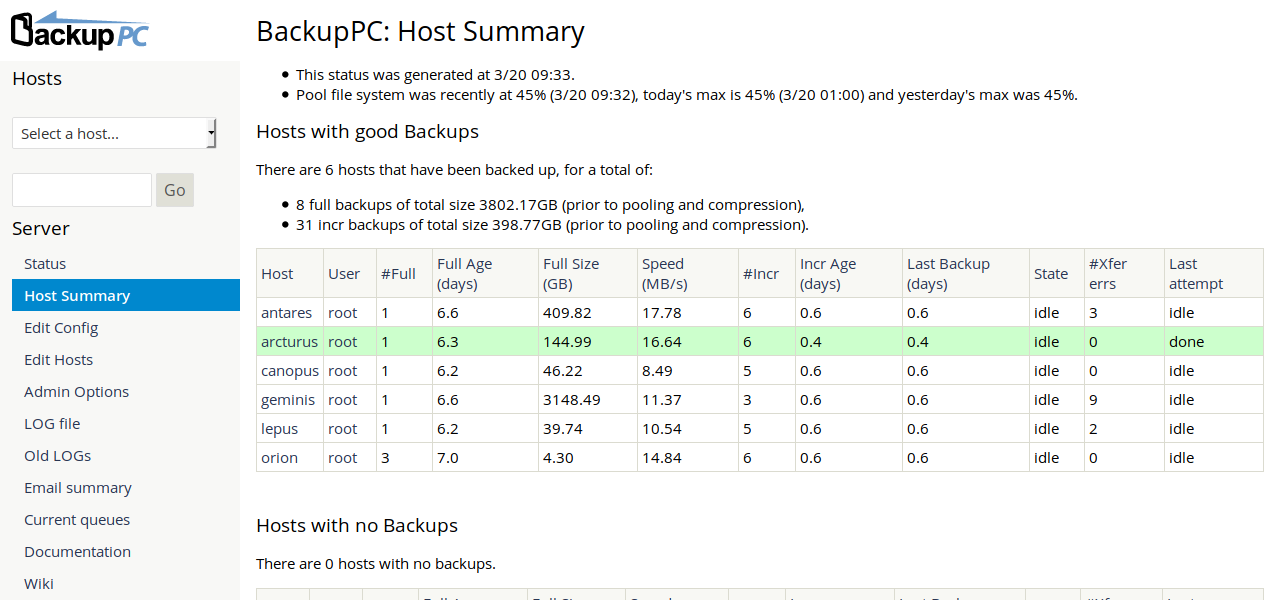
\includegraphics[height=9\baselineskip]{./assets/y04s01-infosec-lab-01-03-p20.png}
				\caption{Огляд сервера~\textenglish{BackupPC}}
				\label{fig:04-backuppc-01-01}
			\end{figure}

			\begin{figure}[!htbp]
				\centering
				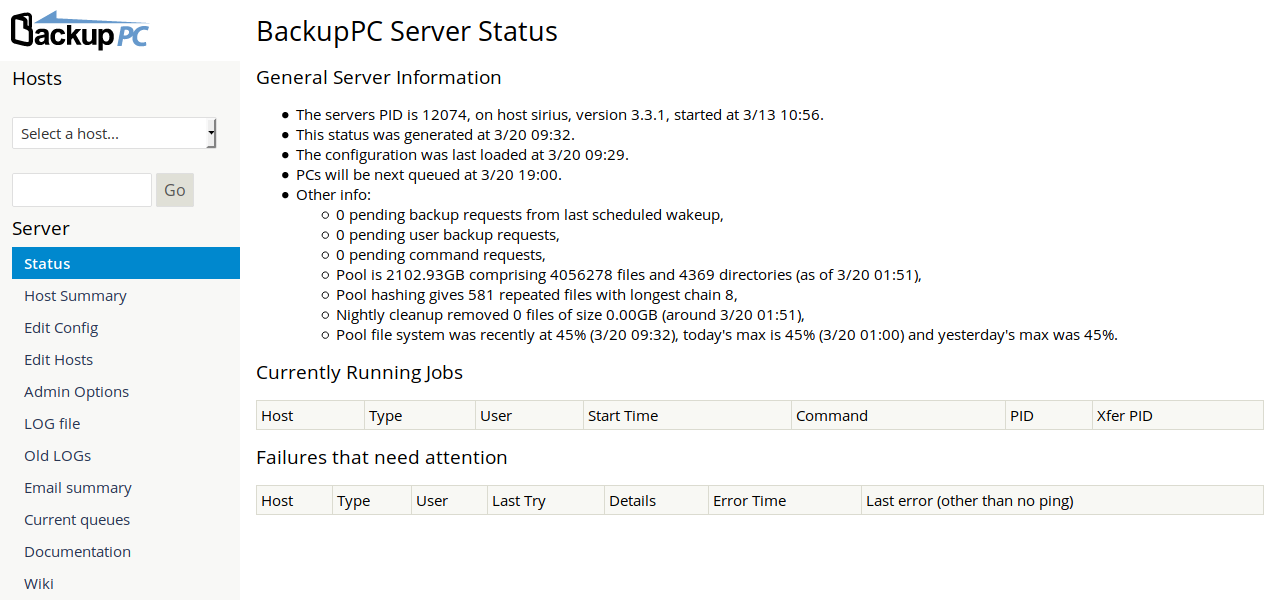
\includegraphics[height=9\baselineskip]{./assets/y04s01-infosec-lab-01-03-p21.png}
				\caption{Огляд хоста~\textenglish{BackupPC}}
				\label{fig:04-backuppc-01-02}
			\end{figure}

			\begin{figure}[!htbp]
				\centering
				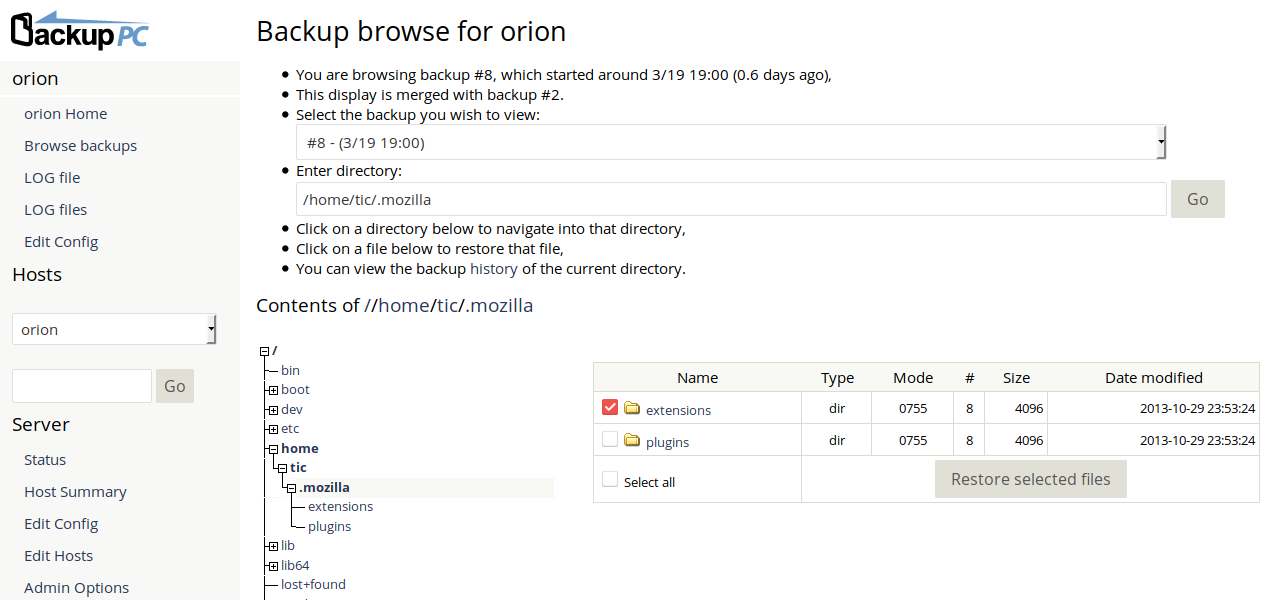
\includegraphics[height=9\baselineskip]{./assets/y04s01-infosec-lab-01-03-p22.png}
				\caption{Огляд резервних копій~\textenglish{BackupPC}}
				\label{fig:04-backuppc-01-03}
			\end{figure}

			\begin{figure}[!htbp]
				\centering
				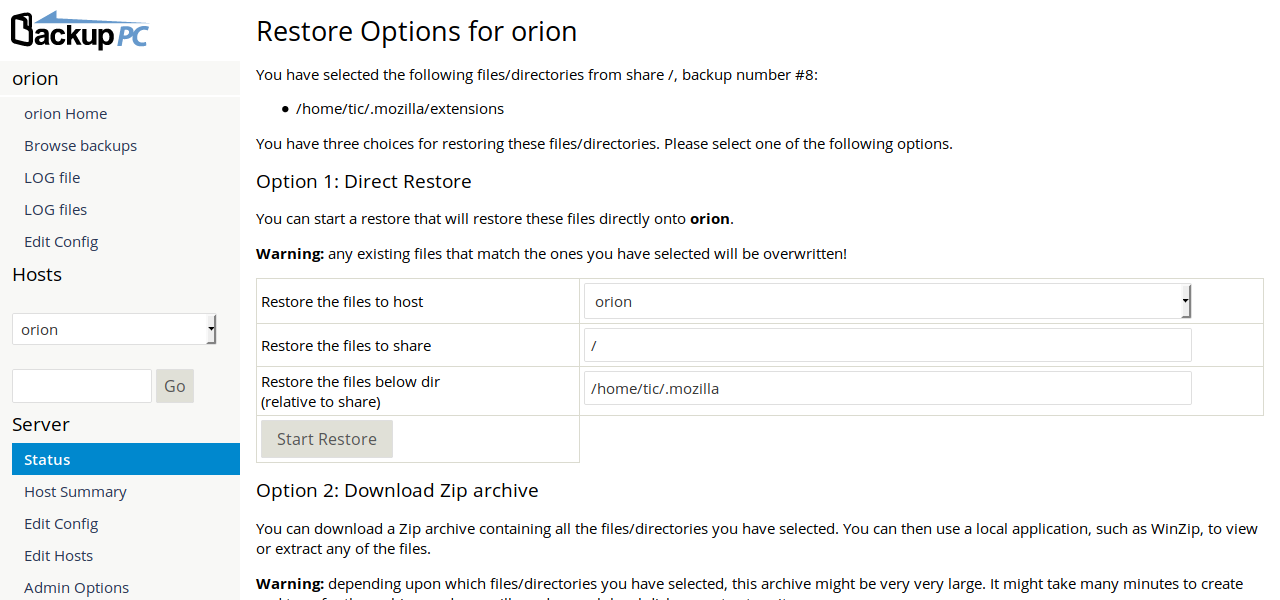
\includegraphics[height=9\baselineskip]{./assets/y04s01-infosec-lab-01-03-p23.png}
				\caption{Відновлення резервних копій~\textenglish{BackupPC}}
				\label{fig:04-backuppc-01-04}
			\end{figure}

			\begin{figure}[!htbp]
				\centering
				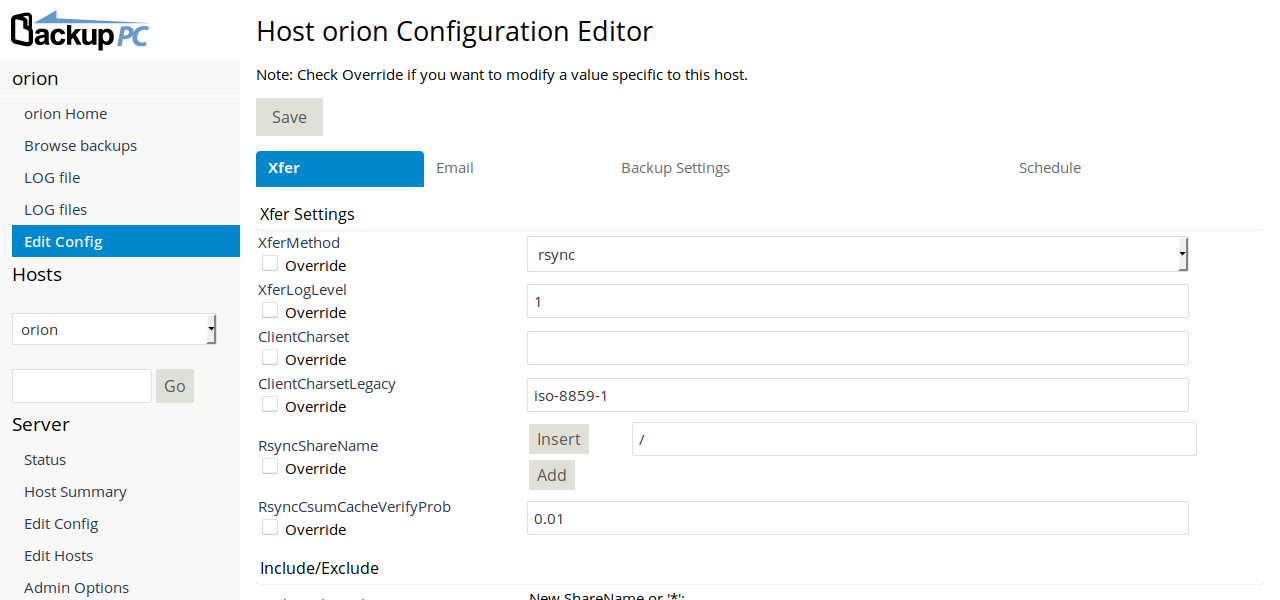
\includegraphics[height=9\baselineskip]{./assets/y04s01-infosec-lab-01-03-p24.png}
				\caption{Налаштування хоста~\textenglish{BackupPC}}
				\label{fig:04-backuppc-01-05}
			\end{figure}

	\section{Висновок}
		Виконуючи дану лабораторну роботу, ми ознайомились з основними принципами застосування резервного копіювання інформації у складі заходів захисту інформації.

\end{document}
